\documentclass[svgnames]{beamer}

\usetheme{Madrid}
\usecolortheme{seahorse}
\usepackage{multirow}

%%%<
\newcommand{\backupbegin}{
   \newcounter{finalframe}
   \setcounter{finalframe}{\value{framenumber}}
}
\newcommand{\backupend}{
   \setcounter{framenumber}{\value{finalframe}}
}
\usepackage{verbatim}
\usepackage{caption}
\setbeamertemplate{navigation symbols}{}
\useinnertheme{rectangles}
\usepackage{varwidth}
\usepackage{xparse}
\usepackage{appendixnumberbeamer}
\usepackage[ruled, vlined, longend]{algorithm2e}
\beamertemplatenavigationsymbolsempty
\usepackage[many]{tcolorbox}
\usetikzlibrary{decorations.pathmorphing}
\usetikzlibrary{fadings,shapes.arrows,shadows,shapes.callouts}   
\usepackage[absolute,overlay]{textpos}
\usepackage{listings}
\lstset {
  backgroundcolor=\color{white},
  basicstyle=\ttfamily\footnotesize,
  numbers=left,numberstyle=\tiny,numbersep=5pt,
  emph={proc, fun, let, send, consume, global, type, record, if, else,
    in, not, foldt, return, on, ordering, by, as, or },
  emphstyle={\bfseries},
  literate = {=>}{{\bf=>}}2
}
\usepackage{graphicx,accents,pinlabel}
\usetikzlibrary{positioning}
\definecolor{paper}{RGB}{239,227,157}
\newtcolorbox{tornpage}{%
    enhanced jigsaw, breakable, % allow page breaks
    frame hidden, % hide the default frame
    overlay={%
        \draw [
            fill=paper, % fill paper
            draw=paper!50!black, % boundary colour
            decorate, % decoration
            decoration={random steps,segment length=2pt,amplitude=1pt},
            drop shadow, % shadow
        ]
        % top line
        (frame.north west)--(frame.north east)--
        % right line
        (frame.north east)--(frame.south east)--
        % bottom line
        (frame.south east)--(frame.south west)--
        % left line
        (frame.south west)--(frame.north west);
    },
    % paragraph skips obeyed within tcolorbox
    parbox=false,
}
%\useoutertheme{default}
%\useinnertheme{rounded}

\titlegraphic{
\begin{center}
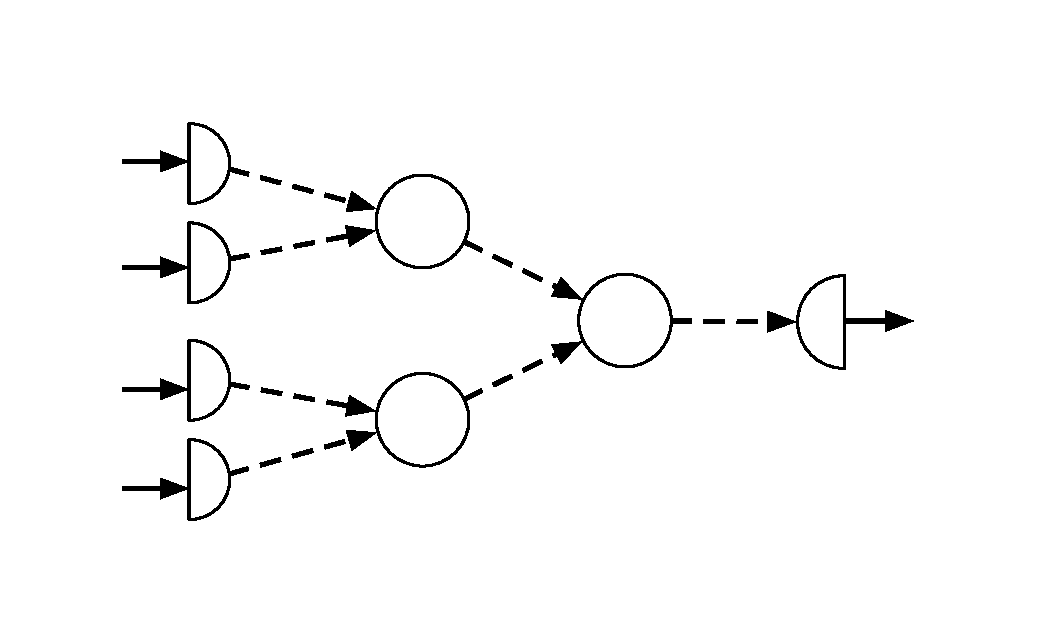
\includegraphics[width=3cm]{hadoop2}%
\end{center}
}

\usepackage{tikz}
\usetikzlibrary{shadows.blur}
\usetikzlibrary{shapes.symbols}
\usetikzlibrary{backgrounds}
\usetikzlibrary{arrows.meta}
\usetikzlibrary{shapes,snakes}
\usetikzlibrary{fit,calc,shadows}
\setbeamercolor{section in head/foot}{bg=white, fg=black}
%\beamertemplateshadingbackground{black!10}{blue!15}
\makeatletter
\setbeamertemplate{footline}
{
  \leavevmode%
  \hbox{%
  \begin{beamercolorbox}[wd=.333333\paperwidth,ht=2.25ex,dp=1ex,center]{section in head/foot}%
    \usebeamerfont{author in head/foot}\insertshortauthor~~\beamer@ifempty{\insertshortinstitute}{}{Richard G. Clegg}
  \end{beamercolorbox}%
  \begin{beamercolorbox}[wd=.333333\paperwidth,ht=2.25ex,dp=1ex,center]{section in head/foot}%
    \usebeamerfont{title in head/foot}{Creating synthetic networks}
  \end{beamercolorbox}%
  \begin{beamercolorbox}[wd=.333333\paperwidth,ht=2.25ex,dp=1ex,right]{section in head/foot}%
    \usebeamerfont{date in head/foot}\insertshortdate{}\hspace*{2em}
    \insertframenumber{} / \inserttotalframenumber\hspace*{2ex} 
  \end{beamercolorbox}}%
  \vskip0pt%
}


\tikzstyle{cloudconn} = [draw=black, inner sep=0pt,
       line width=0.25mm,{Latex[length=2.5mm, width=1.5mm]}-{Latex[length=2.5mm, width=1.5mm]}]

\tikzstyle{arrowconn} = [draw=black, inner sep=0pt,
       line width=0.25mm,-{Latex[length=2.5mm, width=1.5mm]}]
\makeatother

\date[Covid 2021 workshop]{Presentation Covid 2021 workshop}

\begin{document}


\frame{

\title[FETA]{Freeing vital research with synthetic network data}

\setcounter{framenumber}{0}

\begin{center}
\Huge{Creating‌ ‌synthetic‌ ‌models‌ ‌from‌ ‌sensitive‌ ‌data‌ ‌--‌ ‌preparing‌ ‌for‌ ‌future‌‌
epidemics}


\vspace{0.2cm}

\inserttitlegraphic

\vspace{0.2cm}

\scriptsize{\raggedright
{\color{blue} Presenter: }Richard G. Clegg,  \\}
\scriptsize{\raggedright
%Work joint with the {\color{blue} Network-as-a-Service project}.  \\
{
    {\color{blue} FETA written by Naomi Arnold and Richard Clegg}
}

%\tiny{(Prepared using \LaTeX \;and beamer.)}
\end{center}
}

\tikzset{onslide/.code args={<#1>#2}{%
  \only<#1>{\pgfkeysalso{#2}} % \pgfkeysalso doesn't change the path
}}
\tikzset{temporal/.code args={<#1>#2#3#4}{%
  \temporal<#1>{\pgfkeysalso{#2}}{\pgfkeysalso{#3}}{\pgfkeysalso{#4}} % \pgfkeysalso doesn't change the path
}}

\tikzstyle{platform} = [draw=black,shade, 
      anchor=south west,
      align= center,
      top color=blue!40,
      bottom color=blue!5,
      rounded corners=6pt,
      blur shadow={shadow blur steps=5},
      font = \footnotesize]

\section{Introduction}


\tikzstyle{box} = [draw=black,shade, 
      font = \footnotesize,
      align= center,
      top color=blue!40,
      bottom color=blue!5,
      rounded corners=3pt,
      blur shadow={shadow blur steps=5}]

\tikzstyle{box2} = [draw=black,shade, 
      font = \footnotesize,
      align= center,
      top color=red!40,
      bottom color=red!5,
      rounded corners=3pt,
      blur shadow={shadow blur steps=5}]

\tikzstyle{net con} = [draw=black,ultra thick,->]

\frame{
\frametitle{Synthetic graph data: an unmissable opportunity}

\begin{block}{Genuinely important problem}
Network data never more important. Disease transmission, fraud in finance, hate in social networks. Network data never harder to obtain. 
\end{block}
\pause
%\begin{block}{Put synthetic networks on the same footing as time series}
%Time series analysis has standard theoretical models (ARIMA, FARIMA, ARCH, GARCH or TGAN), well known libraries (in python, R, matlab) to generate these models and companies which do this as a service. 
%\end{block}
\pause
\begin{block}{Improve world-leading open source synthetic network software }
FETA v3.0 open source software (MIT licence) creates synthetic networks. Needs further development and commercial use cases to drive adoption. 
\end{block}
\pause
\begin{block}{Clear route to commercial use}
Good contacts with commercial organisations interested in temporal network modelling. Direct route to having software used. 
\end{block}

}

\frame{
    
    \frametitle{Synthetic network data: The problem}
\begin{block}{Isle of Wight Covid App data}
May 2020: trial UK Covid tracking app released on the Isle of Wight.  \\
Data collected: when users encountered each other (network of encounters), when people tested positive for Covid (spread of disease over network). 
\end{block}
\pause
\begin{block}{Invaluable network data that can never be used}
Uses: Understanding disease spread, understanding transmission network, tuning covid app, testing vaccine strategies. \\ 
If researchers had access could revolutionise understanding.
\end{block}
\pause
\begin{itemize}
\item Use case: Financial data sets (network of transactions) --  detecting fraud, money laundering, tracing stolen money. 
\item Use case: Social network (network of interactions) -- spread of hate, harassment, fake news, misinformation. 
\end{itemize}

}



\definecolor{lavander}{cmyk}{0,0.48,0,0}
\definecolor{violet}{cmyk}{0.79,0.88,0,0}
\definecolor{burntorange}{cmyk}{0,0.52,1,0}

\def\lav{lavander!90}
\def\oran{orange!30}

\tikzstyle{peers}=[draw,circle,violet,bottom color=\lav,
                  top color= white, text=violet,minimum width=10pt]
\tikzstyle{superpeers}=[draw,circle,burntorange, left color=\oran,
                       text=violet,minimum width=10pt]
\tikzstyle{legendsp}=[rectangle, draw, burntorange, rounded corners,
                     thin,bottom color=\oran, top color=white,
                     text=burntorange, minimum width=1.5cm]
\tikzstyle{legendp}=[rectangle, draw, violet, rounded corners, thin,
                     bottom color=\lav, top color= white,
                     text= violet, minimum width= 1.5cm]
\tikzstyle{legend_general}=[rectangle, rounded corners, thin,
                           burntorange, fill= white, draw, text=violet,
                           minimum width=1.5cm, minimum height=0.4cm]

\tikzfading[name=arrowfading, top color=transparent!0, bottom color=transparent!95]
\tikzset{arrowfill/.style={#1,general shadow={fill=black, shadow yshift=-0.8ex, path fading=arrowfading}}}
\tikzset{arrowstyle/.style n args={3}{draw=#2,arrowfill={#3}, single arrow,minimum height=#1, single arrow,
single arrow head extend=.3cm,}}

\NewDocumentCommand{\tikzfancyarrow}{O{2cm} O{FireBrick} O{top color=OrangeRed!20, bottom color=Red} m}{
\tikz[baseline=-0.5ex]\node [arrowstyle={#1}{#2}{#3}] {#4};
}


\frame{
\frametitle{Synthetic network data: high level description}


\begin{block}{Synthetic network data}
\begin{itemize}
\item Take an original \alert{target} network.
\item Find algorithmic construction rules that match this network.
\item Grow network (or networks) from these rules.
\end{itemize}
\end{block}

\begin{tikzpicture}
\draw[white] (-2,-3) rectangle (10,2);
\node <2-> at (-0.2,0) {
\begin{minipage}{0.8\textwidth}
\begin{tikzpicture}[auto, thick]
 
  % Place super peers and connect them
  \foreach \place/\name in {{(0,-0.5)/a}, {(1,0)/b}, {(1,1)/c}, {(0,1)/d},
           {(-1,0)/e}}
    \node[superpeers] (\name) at \place {};
  \foreach \source/\dest in {a/b, a/c, a/d, b/c, c/d,a/e,d/e}
    \path (\source) edge (\dest);
   %
   % Place normal peers
  \foreach \pos/\i in {above left of/1, left of/2, below left of/3}
    \node[peers, \pos = e] (e\i) {};
   \foreach \speer/\peer in {e/e1,e/e2,e/e3}
    \path (\speer) edge (\peer);
   %
   %
   \foreach \pos/\i in {above right of/1, right of/2, below right of/3}
    \node[peers, \pos =b ] (b\i) {};
   \foreach \speer/\peer in {b/b1,b/b2,b/b3}
   \path (\speer) edge (\peer);
   %
   \node[peers, above of=d] (d1){};
   \path (d) edge (d1);
   %
   \foreach \pos/\i in {below left of/1, below of/2}
   \node[peers, \pos =a ] (a\i) {};
   \foreach \speer/\peer in {a/a1,a/a2}
   \path (\speer) edge (\peer);
\end{tikzpicture}
\end{minipage}
};

\node<3-> at (1,0) {
\tikzfancyarrow[3cm]{$p_i = k d_i^{\alpha}$}

};

\node <4-> at (7.5,0) {
\begin{minipage}{0.8\textwidth}
\begin{tikzpicture}[auto, thick]
  % Place super peers and connect them
  \foreach \place/\name in {{(0,-0.4)/a}, {(0.9,0.2)/b}, {(0.7,1.3)/c}, {(0.3,1.2)/d},
           {(-1.2,0.3)/e}}
    \node[superpeers] (\name) at \place {};
  \foreach \source/\dest in {a/b, a/c, a/d, b/c, c/d,a/e,d/e}
    \path (\source) edge (\dest);
   %
   % Place normal peers
  \foreach \pos/\i in {above left of/1, left of/2}
    \node[peers, \pos = e] (e\i) {};
   \foreach \speer/\peer in {e/e1,e/e2}
    \path (\speer) edge (\peer);
   %
   %
   \foreach \pos/\i in {above right of/1, right of/2}
    \node[peers, \pos =b ] (b\i) {};
   \foreach \speer/\peer in {b/b1,b/b2}
   \path (\speer) edge (\peer);
   %
   \node[peers, above of=d] (d1){};
   \path (d) edge (d1);
   %
   \foreach \pos/\i in {below left of/1, below right of/2}
   \node[peers, \pos =a ] (a\i) {};
   \foreach \speer/\peer in {a/a1,a/a2}
   \path (\speer) edge (\peer);
\end{tikzpicture}
\end{minipage}
};

\end{tikzpicture}

}


\frame{
    \frametitle{Alternatives to synthetic network data?}
\centering{
\begin{tikzpicture}%[show background grid]
\draw[white] (-5.5,-3.5) rectangle (5.5,3.5);
\node <1-> at (0,0) {
\begin{minipage}{0.8\textwidth}
\begin{block}{Anonymise}
Release the data anonymised so there are no privacy concerns. \\
Allows data to be open and available for research.
\end{block}

    
\begin{block}{Guarantee to keep data secure}
Release data to individual researchers under an NDA (non disclosure agreement). 
\end{block}
\pause
These routes to sharing data present clear danger with the most private (most valuable) data.
Network data is incredibly hard to anonymise well. 
\end{minipage}
};

\node <3-> at (-2,0) {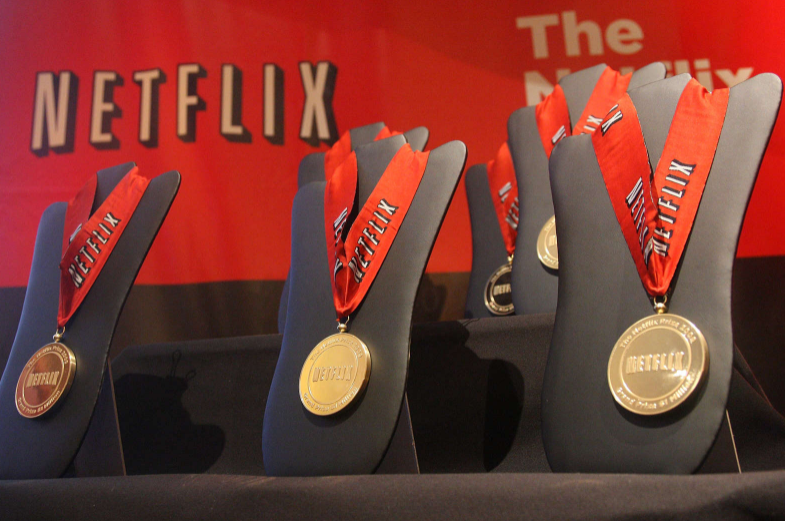
\includegraphics[width=7cm,angle=20]{netflix_prize}};
\node <4-> at (2,2) {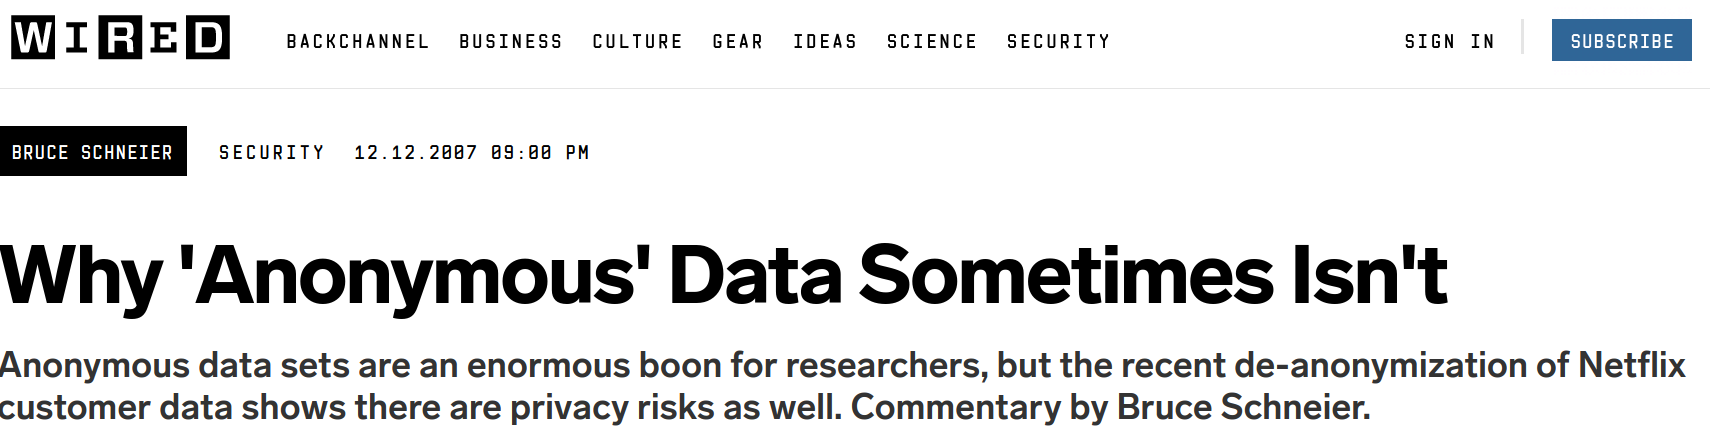
\includegraphics[width=8cm,angle=-10]{wired_netflix}};
\node <5-> at (-1,0) {
\includegraphics[width=8cm,angle=-30]{camb_priv}};
\node <6-> at (0,0) {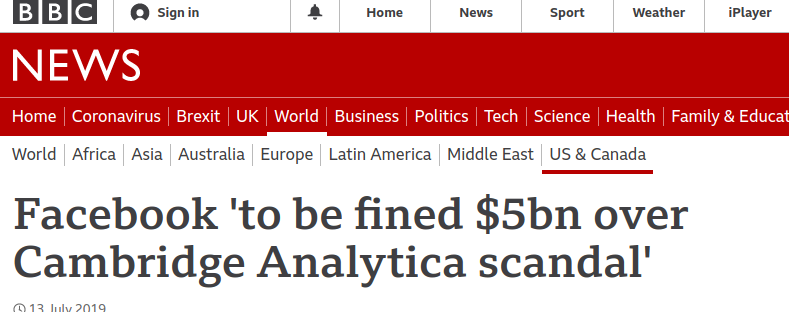
\includegraphics[width=6cm,angle=40]{camb_priv2}};
\end{tikzpicture}

}

}

\frame{
\frametitle{Proposal in a nutshell}
Twelve month project with one postdoctoral researcher (at QMUL). 
\begin{block}{Develop an existing tool for synthetic network data}
FETA (Framework for Evolving Topology Analysis) is an existing open source (MIT licence) tool developed at QMUL. We will:
\begin{itemize}
\item Specialise for use cases in finance (crypto) and social networks.
\item Identify extra use cases at Turing and Accenture.
\item Produce reference synthetic networks for these use cases.
\end{itemize}
\end{block}
\pause
\begin{itemize}
\item Previous ATI project Raphtory develop PhD software led to successful spin out company (Chorograph $\rightarrow$ Pometry).
\item Working with commercial partners in cryptocurrency and social networks area.
\end{itemize}
}

\frame{
    \frametitle{FETA project team}

\begin{tikzpicture}%[show background grid]
\draw[white] (-5,-3) rectangle (5,3);
\node  [inner sep=0pt] at (-4,0) (fc) {\includegraphics[width=1.3cm]{felix}};
\node[align=center] [below= 1pt of fc]  {Felix Cuadrado \\ CoI (QMUL) \\ Expert Graph Systems};
\node [inner sep=0pt] at (0,1.5) (rc) {\includegraphics[width=1.3cm]{rich}};
\node[align=center] [above= 1pt of rc]  {Richard Clegg \\ PI (QMUL) \\ Creator of FETA};
\node [inner sep=0pt] at (4,0) (na) {\includegraphics[width=1.3cm]{naomi}};
\node[align=center] [below= 1pt of na]  {Naomi Arnold \\ PDRA (QMUL) \\ Programmer of FETA};
\node [inner sep=0pt] at (0,-1.5) (ab) {\includegraphics[width=1.3cm]{andrea}};
\node[align=center] [below= 1pt of ab]  {Andrea Baronchelli \\ CoI (City) \\ Expert Finance networks};
\path[draw](rc) edge[cloudconn] (na);
\path[draw] (rc) edge[cloudconn] (fc);
\path[draw] (na) edge[cloudconn] (fc);
\path[draw] (ab) edge[cloudconn] (fc);
\path[draw] (ab) edge[cloudconn] (na);
\path[draw] (ab) edge[cloudconn] (rc);
\end{tikzpicture}
}


\frame{
\frametitle{State of the art synthetic network data}

\begin{block}{Link Data Benchmark Council (project partner)}
LDBC widely used industry standard for synthetic social networks. Software produces synthetic social network data with information about users/posts but with extremely simple graph structure.
\end{block}

\begin{block}{Complex networks based models}
Based on extremely simple mathematical principles. Examples:
\begin{itemize}
\item Random (Erd\H{o}s--Renyi) -- connect new nodes at random.
\item Barab\'{a}si--Albert -- connect new nodes with a probability proportional to node degree.
\item Triangle closure (Jackson) -- connect new node to a random node and a ``friend" of that random node. 
\end{itemize}
Interesting, mathematically tractable but not realistic. 
\end{block}
}



\frame{
\frametitle{FETA: Framework for Evolving Topology Analysis}
\centering{
\begin{tikzpicture}
\node at (0,0) {\begin{minipage}{\textwidth}
\begin{block}{Creates networks from mixtures of models}
Example: model is 50\% Barab\'{a}si--Albert and 50\% Erd\H{o}s--Renyi. These mixtures can vary in time.
\end{block}

\begin{block}{Assess mathematical likelihood against a target observed network}
Which mixture of models $X$, $Y$ and $Z$ is most likely as an explanation of observed network $N$?
Is the model improved if this mixture changes in time?
\end{block}

\begin{block}{Easily allow development of new network model components}
Quick to add in new models for testing. They can then be combined as with the other model components.
\end{block}
\end{minipage}
};
\node<2->[] at (-3.0,-1.2) {
\begin{minipage}{0.5\textwidth}
\pgfmathsetseed{23654}
\begin{tornpage}    
    Likelihood based assessment of Dynamic Networks\\
    \bf{J. Network Sci. 2016}
\end{tornpage}
\end{minipage}};
\node<3->[] at (3.0,-1.2) {
\begin{minipage}{0.5\textwidth}
\pgfmathsetseed{23654}
\begin{tornpage}    
    Likelihood based approach to discriminate mixtures
    of network models...\\
    \bf{Nature Sci. Rep 2021}
\end{tornpage}
\end{minipage}};
\node<4->[] at (0,2) {
\begin{minipage}{0.5\textwidth}
\pgfmathsetseed{23654}
\begin{tornpage}    
    Open source software\\
    \bf{github.com/narnolddd/FETA3}
\end{tornpage}
\end{minipage}};
\end{tikzpicture}
}
}

\frame{
\frametitle{Producing synthetic networks with FETA}
\centering{
\begin{tikzpicture}%[show background grid]
\draw[white] (-1,-1) rectangle (10,7);
\node<1->[box] at (0.5,6.5) (ba) {Barab{\'a}si--Albert \\ model};
\node<1->[box] at (4.5,6.5) (er) {Random model};
\node<1->[box] at (8.5,6.5) (tri) {Triangle model};
\node<1->[box] at (0.5,3.0) (targ){Target Network \\ for synthesis};
\node<2->[box] at (4.5,3.0) (feta){FETA analysis};
\draw<2-> [net con] (ba) -- (feta);
\draw<2-> [net con] (er) -- (feta);
\draw<2-> [net con] (tri) -- (feta);
\draw<2-> [net con] (targ) -- (feta);
\node<3->[box] at (4.5,0.5) (opt){Maximally likely\\ model combination};
\draw<3-> [net con] (feta) -- (opt);
\node<4->[box] at (8.5,0.5) (net){Synthetic network \\ generation};
\draw<4-> [net con] (opt) -- (net);
\draw<5-> [black, fill=green,opacity=0.2] (-1,4.5) rectangle (6,2.5);
\node<5-> at (1,4) {Stays private};
\draw<5-> [black, fill=blue,opacity=0.2] (3,2) rectangle (10,0);
\node<5-> at (7,1.7) {Released to world};
\node<5-> at (6.8,1.3) {(10s/100s bits of info)};
\end{tikzpicture}
}
}


\frame{
\frametitle{Potential beneficiaries -- commercial}

\begin{itemize}
\item Link Data Benchmark Council (social networks)
\begin{itemize}
\item Interactions will mutually improve products.
\end{itemize} 
\item Chainalysis and Mishcon de Reya (blockchain)
\begin{itemize}
\item Will benefit from analysis and ability to release sensitive data.
\end{itemize}
\item Pometry (previously Chorograph) (big data analysis)
\begin{itemize}
\item Spin out developed from previous Turing project Raphtory. Currently closing \pounds 2 million seed funding on graph networks.
\end{itemize}
\item Moogsoft (Artificial Intelligence/Computer networks)
\begin{itemize}
\item Uses networks from FETA, sponsoring PhD involving FETA. 
\end{itemize} 
\item Accenture (consultancy)
\begin{itemize}
\item We will seek extra project partners among Accenture clients interested in state-of-the-art network data.
\item Potential benefit for Accenture and client organisations.
\end{itemize}
\end{itemize}

}

\frame{
\frametitle{Potential beneficiaries -- wider}

\begin{itemize}
\item Complex networks research enabled by synthetic data
\begin{itemize}
\item Conferences right now are full of potentially ground-breaking research with no data to support the assertions. 
\item A small number of well-regarded synthetic data sets in finance, social networks, health (amongst others) could be game changing. 
\end{itemize} 
\item Longer term public benefits
\begin{itemize}
\item Social networks -- improved understanding of hate and misinformation.
\item Financial networks -- detection of fraud and money laundering.
\item Health -- increased understanding of disease transmission and mitigation strategies.
\item Other areas -- very general approach working with any network to better understand and model it.
\end{itemize}
\end{itemize}

}

\frame{
\frametitle{Summary of opportunity}

\begin{block}{Timely problem}
Valuable network data is often collected but also often associated with major privacy concerns. No standard tool for synthetic network data creation exists. 
\end{block}
\pause
%\begin{block}{Put synthetic networks on the same footing as time series}
%Time series analysis has standard theoretical models (ARIMA, FARIMA, ARCH, GARCH or TGAN), well known libraries (in python, R, matlab) to generate these models and companies which do this as a service. 
%\end{block}
\begin{block}{A small investment can make a huge difference}
FETA v3.0 is ``nearly there" and already does things that no other software can do in a space that is very important.
\end{block}
\pause
\begin{block}{Right team, right collaborators}
The team is world-leading in this area and has a great set of collaborators in the use case areas. 
\end{block}

}

\appendix
\backupbegin

\frame{
\frametitle{FETA analysis of Enron email network}
\centering{
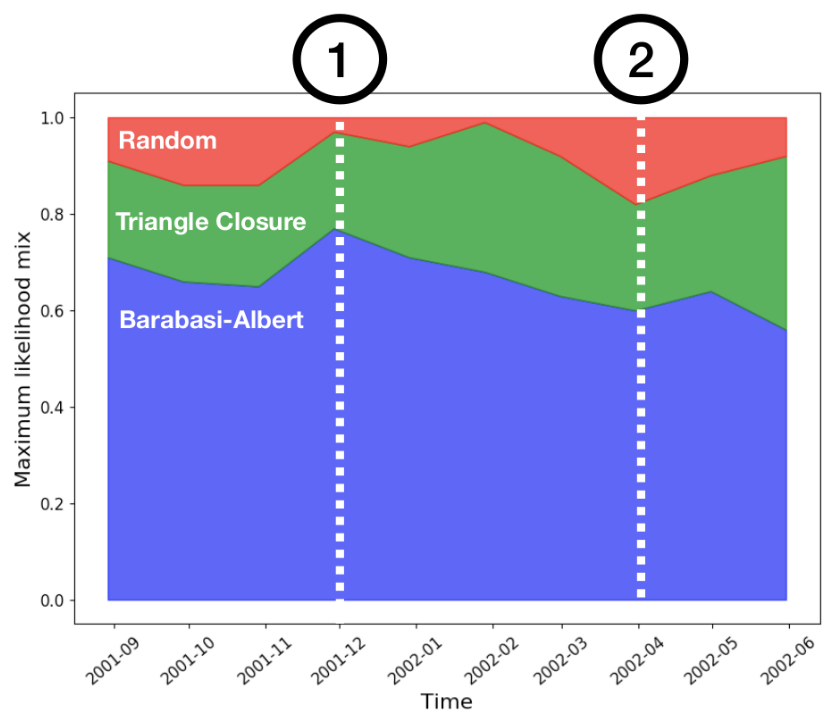
\includegraphics[height=0.7\textheight]{enron}
\begin{enumerate}
\item Enron files for bankruptcy.
\item Auditor pleads guilty of obstruction.
\end{enumerate}
}
}
\backupend


%\frame[noframenumbering]{
%\frametitle{Project team}

%\begin{itemize}
%\item Richard Clegg (Queen Mary) -- principal investigator
%\begin{itemize}
%\item Originated the FETA idea wrote FETA version 1 and 2.
%\item Mathematician and statistician specialising in complex networks.
%\end{itemize}
%\item Felix Cuadrado (Queen Mary) -- Co Investigator
%\begin{itemize}
%\item World leading expert in graph analysis at scale.
%\item 
%\end{itemize}
%\item Andrea Baronchelli (City University) -- Co Investigator
%\begin{itemize}
%\item World leading expert in analysis of cryptocurrency networks.
%\item 
%\end{itemize}
%\item Naomi Arnold (Queen Mary) -- Researcher
%\begin{itemize}
%\item Lead programmer on FETA (version 3).
%\item Submitting PhD on FETA and complex networks in August 2021.
%\end{itemize}
%\end{itemize}
%}

\end{document}
